%This work is licensed under the Creative Commons License Attribution 4.0 International (CC-BY 4.0) 
%https://creativecommons.org/licenses/by/4.0/legalcode 
\documentclass[rgb]{standalone}
\usepackage{tkz-euclide}
\begin{document}
	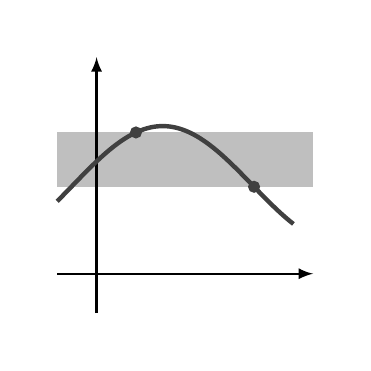
\begin{tikzpicture}[scale=0.5, font=\Large]
		\draw[draw=none] (-1.75,-1.75) -- (-1.75,6.25) -- (6.25,6.25) -- (6.25,-1.75) -- cycle;
		\draw[draw=none, fill, gray, fill opacity=0.5] (-1,{2.25+1.5*sin(120/1.9)}) -- (5.5,{2.25+1.5*sin(120/1.9)}) -- (5.5,{2.25+1.5*sin(345/1.9)}) -- (-1,{2.25+1.5*sin(345/1.9)}) -- cycle; 
		\draw[thick, -latex] (-1,0) -- (5.5,0);
		\draw[thick, -latex] (0,-1) -- (0,5.5);
		\draw[ultra thick,domain=-30:420, smooth, samples=300, variable=\x,darkgray] plot (-45/75+\x/75, {2.25+1.5*sin(\x/1.9)});
		\node[thick, draw=darkgray,circle,fill,darkgray,inner sep=1.25] at (1,{2.25+1.5*sin(120/1.9)}) {};
		\node[thick, draw=darkgray,circle,fill,darkgray,inner sep=1.25] at (4,{2.25+1.5*sin(345/1.9)}) {};
	\end{tikzpicture}
\end{document}